
\documentclass[11pt]{article}\usepackage[]{graphicx}\usepackage[]{color}
% maxwidth is the original width if it is less than linewidth
% otherwise use linewidth (to make sure the graphics do not exceed the margin)
\makeatletter
\def\maxwidth{ %
  \ifdim\Gin@nat@width>\linewidth
    \linewidth
  \else
    \Gin@nat@width
  \fi
}
\makeatother

\definecolor{fgcolor}{rgb}{0.345, 0.345, 0.345}
\newcommand{\hlnum}[1]{\textcolor[rgb]{0.686,0.059,0.569}{#1}}%
\newcommand{\hlstr}[1]{\textcolor[rgb]{0.192,0.494,0.8}{#1}}%
\newcommand{\hlcom}[1]{\textcolor[rgb]{0.678,0.584,0.686}{\textit{#1}}}%
\newcommand{\hlopt}[1]{\textcolor[rgb]{0,0,0}{#1}}%
\newcommand{\hlstd}[1]{\textcolor[rgb]{0.345,0.345,0.345}{#1}}%
\newcommand{\hlkwa}[1]{\textcolor[rgb]{0.161,0.373,0.58}{\textbf{#1}}}%
\newcommand{\hlkwb}[1]{\textcolor[rgb]{0.69,0.353,0.396}{#1}}%
\newcommand{\hlkwc}[1]{\textcolor[rgb]{0.333,0.667,0.333}{#1}}%
\newcommand{\hlkwd}[1]{\textcolor[rgb]{0.737,0.353,0.396}{\textbf{#1}}}%
\let\hlipl\hlkwb

\usepackage{framed}
\makeatletter
\newenvironment{kframe}{%
 \def\at@end@of@kframe{}%
 \ifinner\ifhmode%
  \def\at@end@of@kframe{\end{minipage}}%
  \begin{minipage}{\columnwidth}%
 \fi\fi%
 \def\FrameCommand##1{\hskip\@totalleftmargin \hskip-\fboxsep
 \colorbox{shadecolor}{##1}\hskip-\fboxsep
     % There is no \\@totalrightmargin, so:
     \hskip-\linewidth \hskip-\@totalleftmargin \hskip\columnwidth}%
 \MakeFramed {\advance\hsize-\width
   \@totalleftmargin\z@ \linewidth\hsize
   \@setminipage}}%
 {\par\unskip\endMakeFramed%
 \at@end@of@kframe}
\makeatother

\definecolor{shadecolor}{rgb}{.97, .97, .97}
\definecolor{messagecolor}{rgb}{0, 0, 0}
\definecolor{warningcolor}{rgb}{1, 0, 1}
\definecolor{errorcolor}{rgb}{1, 0, 0}
\newenvironment{knitrout}{}{} % an empty environment to be redefined in TeX

\usepackage{alltt}
\usepackage{graphicx, verbatim}

% \VignetteEngine{knitr::knitr}
% \VignetteIndexEntry{Formatting Examples}
% \VignetteDepends{openxlsx}
% \VignetteKeyword{excel}
% \VignetteKeyword{xlsx}
% \VignetteKeyword{spreadsheet}

\usepackage{geometry}
 \geometry{
 a4paper,
 total={210mm,297mm},
 left=15mm,
 right=15mm,
 top=20mm,
 bottom=20mm,
 }
\IfFileExists{upquote.sty}{\usepackage{upquote}}{}
\begin{document}

\title{Examples}
\author{Alexander Walker\\
\texttt{Alexander.Walker1989@gmail.com}}
\maketitle


\section{Formatting with writeData and writeDataTable}
\begin{verbatim}

## data.frame to write
df <- data.frame("Date" = Sys.Date()-0:4,
                 "Logical" = c(TRUE, FALSE, TRUE, TRUE, FALSE),
                 "Currency" = paste("$",-2:2),
                 "Accounting" = -2:2,
                 "hLink" = "https://CRAN.R-project.org/", 
                 "Percentage" = seq(-1, 1, length.out=5),
                 "TinyNumber" = runif(5) / 1E9, stringsAsFactors = FALSE)

class(df$Currency) <- "currency"
class(df$Accounting) <- "accounting"
class(df$hLink) <- "hyperlink"
class(df$Percentage) <- "percentage"
class(df$TinyNumber) <- "scientific"

## Formatting can be applied simply through the write functions
## global options can be set to further simplify things
options("openxlsx.borderStyle" = "thin")
options("openxlsx.borderColour" = "#4F81BD")

## create a workbook and add a worksheet
wb <- createWorkbook()
addWorksheet(wb, "writeData auto-formatting")

writeData(wb, 1, df, startRow = 2, startCol = 2)
writeData(wb, 1, df, startRow = 9, startCol = 2, borders = "surrounding")
writeData(wb, 1, df, startRow = 16, startCol = 2, borders = "rows")
writeData(wb, 1, df, startRow = 23, startCol = 2, borders ="columns")
writeData(wb, 1, df, startRow = 30, startCol = 2, borders ="all")

## headerStyles
hs1 <- createStyle(fgFill = "#4F81BD", halign = "CENTER", textDecoration = "Bold",
                   border = "Bottom", fontColour = "white")

writeData(wb, 1, df, startRow = 16, startCol = 10, headerStyle = hs1,
          borders = "rows", borderStyle = "medium")

## to change the display text for a hyperlink column just write over those cells
writeData(wb, sheet = 1, x = paste("Hyperlink", 1:5), startRow = 17, startCol = 14)


## writing as an Excel Table

addWorksheet(wb, "writeDataTable")
writeDataTable(wb, 2, df, startRow = 2, startCol = 2)
writeDataTable(wb, 2, df, startRow = 9, startCol = 2, tableStyle = "TableStyleLight9")
writeDataTable(wb, 2, df, startRow = 16, startCol = 2, tableStyle = "TableStyleLight2")
writeDataTable(wb, 2, df, startRow = 23, startCol = 2, tableStyle = "TableStyleMedium21")

openXL(wb) ## opens a temp version

\end{verbatim}

\noindent
The 'tableStyle' argument in writeDataTable can be any ofthe predefined tableStyles in Excel.

\begin{center}
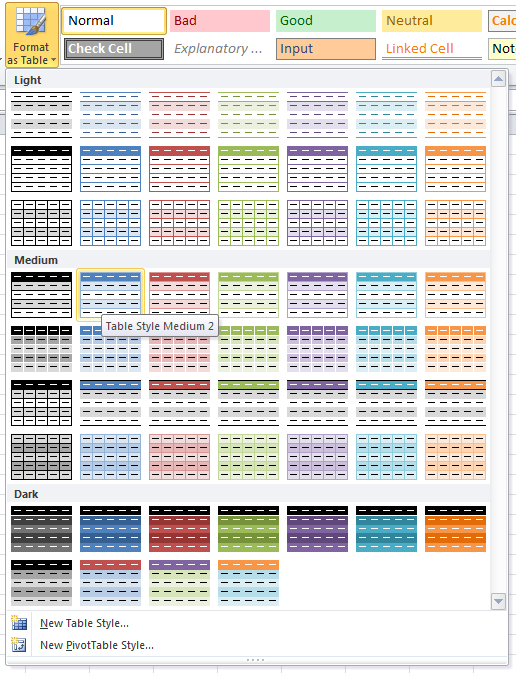
\includegraphics[width=14cm]{tableStyles}
\end{center}

\newpage
\section{Date Formatting}
\begin{verbatim}

# data.frame of dates
dates <- data.frame("d1" = Sys.Date() - 0:4)
for(i in 1:3) dates <- cbind(dates, dates)
names(dates) <- paste0("d", 1:8)

## Date Formatting
wb <- createWorkbook()
addWorksheet(wb, "Date Formatting", gridLines = FALSE)
writeData(wb, 1, dates) ## write without styling

## openxlsx converts columns of class "Date" to Excel dates with the format given by
getOption("openxlsx.dateFormat", "mm/dd/yyyy")

## this can be set via (for example)
options("openxlsx.dateFormat" = "yyyy/mm/dd")
## custom date formats can be made up of any combination of:
##   d, dd, ddd, dddd, m, mm, mmm, mmmm, mmmmm, yy, yyyy

## numFmt == "DATE" will use the date format specified by the above
addStyle(wb, 1, style = createStyle(numFmt = "DATE"), rows = 2:11, cols = 1, gridExpand = TRUE) 

## some custom date format examples
sty <- createStyle(numFmt = "yyyy/mm/dd")
addStyle(wb, 1, style = sty, rows = 2:11, cols = 2, gridExpand = TRUE)

sty <- createStyle(numFmt = "yyyy/mmm/dd")
addStyle(wb, 1, style = sty, rows = 2:11, cols = 3, gridExpand = TRUE)

sty <- createStyle(numFmt = "yy / mmmm / dd")
addStyle(wb, 1, style = sty, rows = 2:11, cols = 4, gridExpand = TRUE)

sty <- createStyle(numFmt = "ddddd")
addStyle(wb, 1, style = sty, rows = 2:11, cols = 5, gridExpand = TRUE)

sty <- createStyle(numFmt = "yyyy-mmm-dd")
addStyle(wb, 1, style = sty, rows = 2:11, cols = 6, gridExpand = TRUE)

sty <- createStyle(numFmt = "mm/ dd yyyy")
addStyle(wb, 1, style = sty, rows = 2:11, cols = 7, gridExpand = TRUE)

sty <- createStyle(numFmt = "mm/dd/yy")
addStyle(wb, 1, style = sty, rows = 2:11, cols = 8, gridExpand = TRUE)

setColWidths(wb, 1, cols = 1:10, widths = 23)

## The default date format used in writeData and writeDataTable can be set with:
options("openxlsx.dateFormat" = "dd/mm/yyyy")
writeData(wb, "Date Formatting", dates, startRow  = 8, borders = "rows")
options("openxlsx.dateFormat" = "yyyy-mm-dd")
writeData(wb, "Date Formatting", dates, startRow  = 15)

saveWorkbook(wb, "Date Formatting.xlsx", overwrite = TRUE)
\end{verbatim}





\newpage
\section{DateTime Formatting}
\begin{verbatim}

The conversion from POSIX to Excel datetimes is dependent on the timezone you are in.
If POSIX values are being written incorrectly, try setting the timezone with (for example)
Sys.setenv(TZ = "Australia/Sydney")

dateTimes <- data.frame("d1" = Sys.time() - 0:4*10000)
for(i in 1:2) dateTimes <- cbind(dateTimes, dateTimes)
names(dateTimes) <- paste0("d", 1:4)

## POSIX Formatting
wb <- createWorkbook()
addWorksheet(wb, "DateTime Formatting", gridLines = FALSE)
writeData(wb, 1, dateTimes) ## write without styling

## openxlsx converts columns of class "POSIxt" to Excel datetimes with the format given by
getOption("openxlsx.datetimeFormat", "yyyy/mm/dd hh:mm:ss")

## this can be set via (for example)
options("openxlsx.datetimeFormat" = "yyyy-mm-dd hh:mm:ss")
## custom datetime formats can be made up of any combination of:
## d, dd, ddd, dddd, m, mm, mmm, mmmm, mmmmm, yy, yyyy, h, hh, m, mm, s, ss, AM/PM

## numFmt == "LONGDATE" will use the date format specified by the above
long_date_style <- createStyle(numFmt = "LONGDATE")
addStyle(wb, 1, style = long_date_style, rows = 2:11, cols = 1, gridExpand = TRUE) 

## some custom date format examples
sty <- createStyle(numFmt = "yyyy/mm/dd hh:mm:ss AM/PM")
addStyle(wb, 1, style = sty, rows = 2:11, cols = 2, gridExpand = TRUE)

sty <- createStyle(numFmt = "hh:mm:ss AM/PM")
addStyle(wb, 1, style = sty, rows = 2:11, cols = 3, gridExpand = TRUE)

sty <- createStyle(numFmt = "hh:mm:ss")
addStyle(wb, 1, style = sty, rows = 2:11, cols = 4, gridExpand = TRUE)

setColWidths(wb, 1, cols = 1:4, widths = 30)

## The default date format used in writeData and writeDataTable can be set with:
options("openxlsx.datetimeFormat" = "yyyy/mm/dd hh:mm:ss")
writeData(wb, "DateTime Formatting", dateTimes, startRow  = 8, borders = "rows")

options("openxlsx.datetimeFormat" = "hh:mm:ss AM/PM")
writeDataTable(wb, "DateTime Formatting", dateTimes, startRow  = 15)

saveWorkbook(wb, "DateTime Formatting.xlsx", overwrite = TRUE)
openXL("DateTime Formatting.xlsx")

\end{verbatim}



\newpage
\section{Conditional Formatting}
\begin{verbatim}

wb <- createWorkbook()
addWorksheet(wb, "cellIs")
addWorksheet(wb, "Moving Row")
addWorksheet(wb, "Moving Col")
addWorksheet(wb, "Dependent on 1")
addWorksheet(wb, "Duplicates")
addWorksheet(wb, "containsText")
addWorksheet(wb, "colourScale", zoom = 30)
addWorksheet(wb, "databar")

negStyle <- createStyle(fontColour = "#9C0006", bgFill = "#FFC7CE")
posStyle <- createStyle(fontColour = "#006100", bgFill = "#C6EFCE")

## rule applies to all each cell in range
writeData(wb, "cellIs", -5:5)
writeData(wb, "cellIs", LETTERS[1:11], startCol=2)
conditionalFormatting(wb, "cellIs", cols=1, rows=1:11, rule="!=0", style = negStyle)
conditionalFormatting(wb, "cellIs", cols=1, rows=1:11, rule="==0", style = posStyle)

## highlight row dependent on first cell in row
writeData(wb, "Moving Row", -5:5)
writeData(wb, "Moving Row", LETTERS[1:11], startCol=2)
conditionalFormatting(wb, "Moving Row", cols=1:2, rows=1:11, rule="$A1<0", style = negStyle)
conditionalFormatting(wb, "Moving Row", cols=1:2, rows=1:11, rule="$A1>0", style = posStyle)

## highlight column dependent on first cell in column
writeData(wb, "Moving Col", -5:5)
writeData(wb, "Moving Col", LETTERS[1:11], startCol=2)
conditionalFormatting(wb, "Moving Col", cols=1:2, rows=1:11, rule="A$1<0", style = negStyle)
conditionalFormatting(wb, "Moving Col", cols=1:2, rows=1:11, rule="A$1>0", style = posStyle)

## highlight entire range cols X rows dependent only on cell A1
writeData(wb, "Dependent on 1", -5:5)
writeData(wb, "Dependent on 1", LETTERS[1:11], startCol=2)
conditionalFormatting(wb, "Dependent on 1", cols=1:2, rows=1:11, rule="$A$1<0", style = negStyle)
conditionalFormatting(wb, "Dependent on 1", cols=1:2, rows=1:11, rule="$A$1>0", style = posStyle)

## highlight duplicates using default style
writeData(wb, "Duplicates", sample(LETTERS[1:15], size = 10, replace = TRUE))
conditionalFormatting(wb, "Duplicates", cols = 1, rows = 1:10, type = "duplicates")

## cells containing text
fn <- function(x) paste(sample(LETTERS, 10), collapse = "-")
writeData(wb, "containsText", sapply(1:10, fn))
conditionalFormatting(wb, "containsText", cols = 1, rows = 1:10, type = "contains", rule = "A")

## colourscale colours cells based on cell value
df <- read.xlsx(system.file("readTest.xlsx", package = "openxlsx"), sheet = 4)
writeData(wb, "colourScale", df, colNames=FALSE)  ## write data.frame

## rule is a vector or colours of length 2 or 3 (any hex colour or any of colours())
## If rule is NULL, min and max of cells is used. Rule must be the same length as style or NULL.
conditionalFormatting(wb, "colourScale", cols=1:ncol(df), rows=1:nrow(df),
   style = c("black", "white"), 
   rule = c(0, 255), 
   type = "colourScale")

setColWidths(wb, "colourScale", cols = 1:ncol(df), widths = 1.07)
setRowHeights(wb, "colourScale", rows = 1:nrow(df), heights = 7.5) 

## Databars
writeData(wb, "databar", -5:5)
conditionalFormatting(wb, "databar", cols = 1, rows = 1:12, type = "databar") ## Default colours

saveWorkbook(wb, "conditionalFormattingExample.xlsx", TRUE)

openXL(wb)


\end{verbatim}


\newpage
\section{Numeric Formatting}
\begin{verbatim}

numeric columns styling can be set using the numFmt parameter in createStyle or a default can be 
set with, for example, options("openxlsx.numFmt" = "#,#0.00")

options("openxlsx.numFmt" = NULL)
wb <- createWorkbook()
addWorksheet(wb, "Sheet 1")
df <- data.frame(matrix(12.987654321, ncol = 7, nrow = 5)) ## data.frame to write
df[ ,6:7] <- df[ ,6:7]*1E6

## Set column 1 class to "comma" to get comma separated thousands
class(df$X1) <- "comma"

writeData(wb, 1, df)
s <- createStyle(numFmt = "0.0")
addStyle(wb, 1, style = s, rows = 2:6, cols = 2, gridExpand = TRUE)

s <- createStyle(numFmt = "0.00")
addStyle(wb, 1, style = s, rows = 2:6, cols = 3, gridExpand = TRUE)

s <- createStyle(numFmt = "0.000")
addStyle(wb, 1, style = s, rows = 2:6, cols = 4, gridExpand = TRUE)

s <- createStyle(numFmt = "#,##0")
addStyle(wb, 1, style = s, rows = 2:6, cols = 5, gridExpand = TRUE)

s <- createStyle(numFmt = "#,##0.00")
addStyle(wb, 1, style = s, rows = 2:6, cols = 6, gridExpand = TRUE)

s <- createStyle(numFmt = "$ #,##0.00")
addStyle(wb, 1, style = s, rows = 2:6, cols = 7, gridExpand = TRUE)

## set a default number format for numeric columns of data.frames
options("openxlsx.numFmt" = "$* #,#0.00")
writeData(wb, 1, x = data.frame("Using Default Options" = rep(2345.1235, 5)), startCol = 9)

setColWidths(wb, 1, cols = 1:10, widths = 15)

## Using default numFmt to round to 2 dp (Any numeric column will be affected)
addWorksheet(wb, "Sheet 2")
df <- iris; df[, 1:4] <- df[1:4] + runif(1)
writeDataTable(wb, sheet = 2, x = df)
writeData(wb, sheet = 2, x = df, startCol = 7)
writeData(wb, sheet = 2, x = df, startCol = 13, borders = "rows")

## To stop auto-formatting numerics set
options("openxlsx.numFmt" = NULL)
addWorksheet(wb, "Sheet 3")
writeDataTable(wb, sheet = 3, x = df)

openXL(wb)


if (identical(Sys.getenv("NOT_CRAN", unset = "true"), "false")) {
file_list<-list.files(pattern="\\.xlsx",recursive = T)
file_list<-fl[!grepl("inst/extdata",file_list)&!grepl("man/",file_list)]

if(length(file_list)>0){
rm(file_list)
}

}

\end{verbatim}



\end{document}
